\documentclass[11pt]{article}
\usepackage{basecommon}
\usepackage[margin=1.5in, top=1in]{geometry}
\usepackage{graphicx}
\usepackage[backend=bibtex, natbib=true, autocite=superscript, style=authoryear-ibid]{biblatex}
\usepackage{hyperref}
\usepackage{url}
\usepackage{lineno}
\addbibresource{citations_annotated.bib}
\graphicspath{ {images/} }
\usepackage{setspace}
\doublespacing
\title{Chapter 1 (DRAFT)}
\author{Hugh Zabriskie}
\date{3 December 2015}
\begin{document}
\maketitle{}
\linenumbers

\section{A primer on machine learning topics}


\subsection{Supervised machine learning}

In machine learning, a subfield of artificial intelligence, we are concerned with the concept of learning from a dataset. Machine learning can be broadly divided into two categories, supervised and unsupervised learning, and the two have unique goals in learning. In supervised learning, a set of observations is correlated with a set of corresponding outcomes, which become the inputs and outputs of the machine. Supervised learning can be used to \textit{predict} - given a series of known observations and outcomes, learn to predict future outcomes. Consider the task of learning to predict the price of a car given a set of the car's features. By a mathematical "learn-by-example" method, a machine is shown several cars and their known prices, and eventually learns to predict what a car's price might be. Therefore, the primary task is to optimize the machine's \textit{parameters}, denoted by the symbol $\theta$, in order to improve accuracy of predictions. In terms of linear algebra, $\theta$ might be vectors of parameters such that our prediction $p$ is modeled as $f(x) = \theta^T x$. Based on the prediction and the target output, a cost function is evaluated to determine prediction error, and then parameters are updated to decrease error in future predictions.

\subsection{Distributions and classification}

The machine learning algorithms used in this paper commonly accept an input vector (or series of vectors) and output a \textit{distribution} - that is, every possible output is assigned a probability. These distributions are initially unknown, but the objective is to learn to estimate these distributions given a dataset of observations and known outcomes. Mathematically, the objective is to learn the mapping $f: {\cal X} \rightarrow {\cal Y}$, given a set of $n$ examples, such that $f(\boldx) \approx \boldy$. The training data is the data on which the machine learns the correlation, and then the machine's ability to predict future outcomes is evaluated on a separate test dataset. In logistic regression and other classification algorithms used in this paper, the possible outcomes or values of $y$ represent a discrete set of $k$ classes, and the distribution produced by the algorithm represents the probability that $\boldx$ belongs to each class. \\

\subsection{Logistic regression}

The logistic regression is a binary (2-class) classification algorithm with a Bernoulli distribution, where the prediction output $y$ is classified as 1 with probability $p$, and 0 with probability $1-p$. In other words, the logistic regression models $f : {\cal X} \rightarrow {\cal Y} \in \{0,1\}$ \citep[p.~21]{murphy2012machine}. An example would be an input vector that represented information about a patient's symptoms and the output represents a prediction of whether the patient has a certain disease ($y=1$) or not ($y=0$). We say that
\begin{align*}
P(Y = 1 | \boldx, \theta) = \textnormal{Ber}(Y = 1 | f(\boldx) )
\end{align*}

\noin to mean the probability of the random variable $Y$ given an $n$-dimensional input vector $\boldx$ and a weight vector $\theta$ is a Bernoulli distribution given $f(\boldx)$, which represents some linear combination of the inputs. The distribution for $y$ is typically calculated as a linear function of $x$ and $\theta$ in the form $x_1\theta_1 + x_2\theta_2 + ... + x_n\theta_n$. In order to interpret $Y$ as a probability, the sigmoid function $\sigma(\mu)$, or "squashing function" is then applied, which maps any value to the range $[0,1]$.

\begin{figure*}[h]
\caption{The sigmoid function: $\sigma: \reals \rightarrow [0,1]$}
\centering
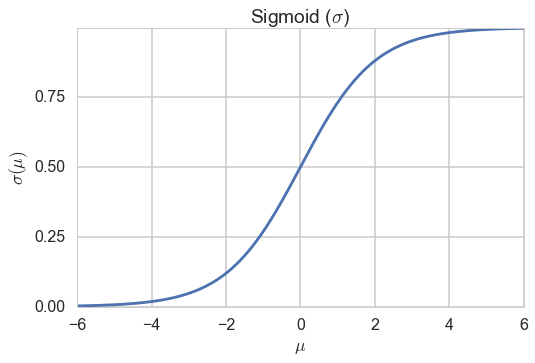
\includegraphics[scale=0.5]{sigmoid}
\end{figure*}


\noin The \textit{hypothesis}, $h_\theta(x)$ given the weights $\theta$, is defined as
\begin{align*}
h_\theta(x) &= \sigma(\theta^Tx) = \sigma \Big(\sum_{i=1}^n \theta_i x_i \Big) \\ 
\Pr(y | x, \theta) &= \Bern(y | h_\theta(x))
\end{align*}

\noin Finally, $y$ is mapped to the discrete binary set $\{0, 1\}$ using a decision boundary $d$, where $0 \leq d \leq 1$.
\begin{align*}
h_\theta(x) \geq d &\to y = 1 \\
h_\theta(x) < d &\to y = 0 \\
\end{align*}

\noin Based on training data, a logistic regression model learns to optimize its predictions for newly observed data by updating the weights $\theta$. Given an observation, a cost function $J$ is used to generate an error metric for the predicted outcome $h_\theta(\boldx)$ based on the "correct" observed outcome. $\theta$ is then updated based on $J(h_\theta(\boldx))$ by a method known as gradient descent. The weights in $\theta$ can be thought of as the control gates for the flow of information, and increasing the value of weight represents an increase in the importance of that information. \\

Multinomial logistic regression is a generalization of logistic regression to the case where we want to handle multiple classes. The objective is to develop a hypothesis to estimate the probability that $\Pr(y = k | x)$ for $k \in 1, \ldots, K$. This is useful in handwritten digit recognition, where $\boldx$ is a numerical representation of an image of a digit, and $y$ is the estimated probability the image represents each of the 10 possible digits (0 - 9). In order to represent $k$ classes, $\theta$ is now a \textit{matrix} of weights, making $\theta^Tx$ a vector. The sigmoid function is replaced with the softmax, which analogously normalizes the distribution $\theta^Tx$ so that the elements of the hypothesis $h_\theta(x)$ sum to 1.

$$h_\theta(x) = \begin{bmatrix}
			P(y = 1| x, \theta) \\
			P(y = 2| x, \theta) \\
			\vdots \\
			P(y = K| x, \theta) \\
			\end{bmatrix}
			= \frac{1}{\sum_{i=1}^K \exp(\theta^{(i)T}x)}
			\cdot \begin{bmatrix}
			\exp(\theta^{(1)T}x) \\
			\exp(\theta^{(2)T}x) \\
			\vdots \\
			\exp(\theta^{(K)T}x) \\
			\end{bmatrix}$$ \\
			
\noin where $\theta$ is represented as

$$\theta = \begin{bmatrix} | && | && | && | \\
		\theta_1 && \theta_2 && \ldots && \theta_K \\ 
		 | && | && | && |
		\end{bmatrix}$$ \\

The most likely classification, or the digit is most likely represented by the image, is selected as the class with the highest estimated probability. Mathematically, $$\argmax_k Pr(y = k| x, \theta)$$


\subsection{Neural Networks}

In this section, I introduce \textit{artificial neural networks}, which are the core machine learning algorithm used in this paper. Neural networks give us a way to understand deeper interactions, and to generate predictions based on a combination of many non-linear functions - a series of cascading smaller decisions to determine a larger decision. They are exceptionally powerful, and by the Universal Approximation Theorem (Cybenko et. al. 1989), a feed-forward neural network with a single hidden layer of finite size is proven to approximate any continuous function bounded by $n$ dimensions with any desired non-zero error \citep{goldberg2015nnlp}. Neural networks are an implementation of multinomial logistic classification, and they are loosely inspired by biological neural networks. Per the analogy, the "neuron" is a unit with a unique weight that accepts scalar inputs and returns a scalar output. Neurons are organized as a serious of layers, the first being the input layer, the last one the output layer, and all intermediary layers being hidden layers. In order to obtain a distribution for the input $\boldx$, $\boldx$ is passed through the network by \textit{forward propagation}. At each step, the neuron multiplies each input by its weight, performs a summation, applies a non-linear function (i.e. the sigmoid function), and then passes the result forward to each neuron in the next layer. Each connection between two neurons also carries a unique weight. This continues until the final output layer, where the resulting layer represents the hypothesis $h_\theta(\boldx)$, often normalized using softmax to transform the output into a discrete distribution over $k$ possible outcomes. Therefore, in a three-layer network, forward propagation over the input vector $\boldx$ can be modeled as follows, with bias terms $\boldb^{(1)}, \boldb^{(2)}$.
\begin{align*}
\boldz^{(1)} &= \boldx \cdot \theta^{(1)} + \boldb^{(1)} \\
\bolda^{(1)} &= \sigma(\boldz^{(1)}) \\
\boldz^{(2)} &= \bolda^{(1)} \cdot \theta^{(2)} + \boldb^{(2)} \\
\bolda^{(2)} &= \sigma(\boldz^{(2)}) \\
h_\theta(x) &= \bolda^{(2)} \cdot \theta^{(3)}
\end{align*}

\begin{figure*}[h]
\caption{Abstract representation of a three-layer neural network architecture, where each circle represents a neuron. $\theta$ controls the flow of information between activation layers.}
\centering
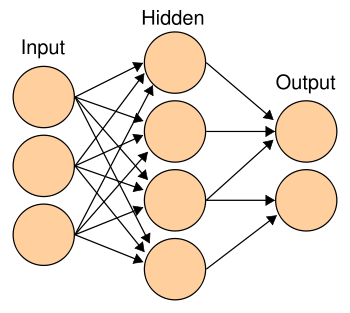
\includegraphics[scale=0.55]{nn}
\end{figure*}

Like the logistic regressions examined earlier, the distribution is dependent on the weights $\theta$. A \textit{cost} is calculated based on a chosen metric of distance (or error) between the estimated distribution and target distribution (the "right answer"), and we can now re-define the objective as the minimization of this cost over the training set. The algorithm for training works by forward propagating each input vector in the training set, using the cost function to estimate the prediction error, and then updating each element of $\theta$ to minimize future error. The prediction-cost-update cycle used in neural networks illustrates the concept learning by example used in supervised learning.



\subsection{Recurrent Neural Networks (RNN)}

Recurrent neural networks (RNNs) provide a solution to a serious limitation of the neural networks described above. The original network accepts a fixed size input vector and produces a fixed size output vector, and as a result, there is a fixed number of computational steps occurring to create each prediction \citep{karpathy2015rnn}. Consequently, the distribution for each input is estimated independently of previous ones, even though as part of the learning process it could be useful to know about previous inputs. In the task of writing a sentence, for example, each word in the sentence is dependent upon the previous ones. RNNs introduce the idea of computational \textit{memory} to store previous decisions, where the hypothesis for input vector $i$ is conditioned upon the hypotheses of previous inputs $h_\theta(\boldx_{i-1})$. The most basic RNN architecture, known as the Elman network, can be modeled as follows:
\begin{align*}
\bolda_i(\boldx) &= \sigma(\boldx_i \cdot \theta^{(1)} + \boldy(\boldx_{i-1}) \cdot \theta^{(2)}) \\
\boldy_\theta(\boldx_i) &= g(\bolda_i(\boldx))
\end{align*}
\noin where $g$ is a non-linear transformation (i.e. $\tanh$, ReLU) \citep[p.~56]{goldberg2015nnlp}. More abstractly, the state at the time $t$ is a function of the input vector $\boldx$ at $t$ and the state vector $\boldy$ at $t-1$. To model this recursive structure, the input to the network is now represented as an \textit{ordered series} of vectors over time. Note that the parameters $\theta$ are shared across all time steps. To train the network, the same procedure for non-recurrent networks applies but now over a sequence of inputs: create a computation graph over time, calculate error for the most recent prediction, and then back-propagate the error across the unfolded network, generating gradients and updating each weight in $\theta$ \citep[p.~63]{goldberg2015nnlp}. \footnote{ Make a new diagram for RNN similar to http://www.hexahedria.com/2015/08/03/composing-music-with-recurrent-neural-networks/ } \\

\begin{figure*}[h]
\centering
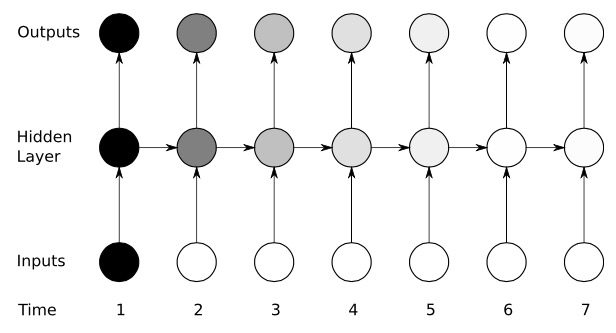
\includegraphics[scale=0.55]{rnn}
\caption{Abstraction of an RNN over a time series. The activation of the neurons in the hidden layer is a function of the input from the previous layer and its own output from the previous computation. }
\end{figure*}

RNNs incorporate previous decisions into their computations and are able to model data as \textit{sequences} of inputs and outputs, and consequently sequences and lists are the natural architecture for input \citep{colah2015lstms}. As a result, RNNs are better able to model contextualized decision-making. Their track record is impressive, and RNNs have been described as "unreasonably effective" on an incredible diversity of tasks, from speech recognition to language translation and image captioning \citep{karpathy2015rnn}.

\subsection{Long Short-Term Memory (LSTM)}

LSTMs are a flavor of RNNs that enhance the memory capabilities of the recurrent network, first introduced by Schmidhuber and Hochreiter (1997) \citep{hochreiter1997long}. In that architecture, feedback is "short-term" in that it is only drawn from the previous computation at time $i-1$, and therefore as more computations occur, the signal from more distant computations is lost. This is known as the "vanishing gradients problem" in the literature \citep[p.~56]{goldberg2015nnlp}, where gradients refer to the updates to $\theta$ that occur during backwards propagation. LSTMs solve this issue by substituting the regular neuron with a \textit{memory cell} that can store those gradients across an arbitrary series of inputs. Information is stored and segregated within the cell by use of multiplicative gate units, such as the input and output gates, that allow information to flow through the cell without affecting other memory contents. A gate $\boldg$ is represented as a $n$-dimensional vector of values in the range $[0,1]$ that is multiplied with a vector $\boldv \in \mathbb{R}^n$, and the result is added as an error signal to a state vector. During training, these gates learn to control the flow of error signal into the input and output by adjusting $\boldg$ (note that a value close to 0 will cause some feature of $\boldv$ to be eliminated). The deeper mathematical foundations for LSTMs are not necessary to understand here, but they have proven to be exceptionally effective models within the RNN family for keeping track of temporally distant events that indicate information about global structure. Eck and Schmidhuber (2002) demonstrated the preliminary effectiveness of LSTMs in the field of music by training a machine to learn and reproduce chord progression in the blues style. They concluded the LSTM was able to learn "both the local structure of melody and the long-term structure of a musical style" \citep{eck2002blues}. More recently, I add another sentence about advances with LSTMs and music.

\begin{figure*}[h]
\centering
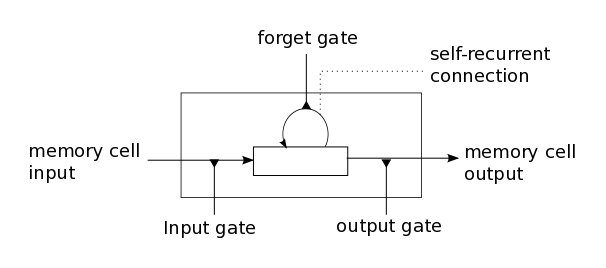
\includegraphics[scale=0.5]{lstm}
\caption{Abstraction of an LSTM memory cell.}
\end{figure*}


\section{An introduction to tonal harmony and the chorale}

In this paper, machine learning algorithms are applied to a data set of four-voices chorales composed by J.S. Bach (herein referred as the "chorales") in order to learn the task of chorale harmonization. In order for the data set to be learned upon, feature spaces must be generated for a set of musical properties that will be fed to the neural networks. To understand these features and their importance in the task of harmonization, a basic understanding of tonal harmony and the properties of the chorales is provided. \\

\citet{cuthbertmusic21} developed the \textsc{music21} Python library as a toolkit for computational musicology, which is used heavily in this paper to manipulate the Bach chorales and transform them into a numerical dataset appropriate for machine learning. \textsc{Music21} adopts an object-oriented design for creating high-level musical objects, which contributes to its ease of use and popularity amongst developers. In introducing the reader to the important building blocks of tonal music and the chorales, I employ a similar high-level \textit{object-oriented} approach in order to illuminate the methods for decomposing a musical score in a collection of high-level objects that can be numerically represented. \\

\subsection{Pitch class, pitch, note}

The fundamental musical object in Western tonal music is the \textit{pitch class}. This system operates over a series of 12 \textit{pitch classes}, some being enharmonic (i.e. C$\sharp$/D$\flat$), meaning that they employ different names depending on musical context such as key signature. \footnote{ We will assume equal temperament.}

\begin{center}
C, C$\sharp$/D$\flat$, D, D$\sharp$/E$\flat$, E, F, F$\sharp$/G$\flat$, G, G$\sharp$/A$\flat$, A, A$\sharp$/B$\flat$, B
\end{center}

A \textit{pitch} is a subclass of the pitch class that identifies a unique frequency. It can be defined as a pitch class with an octave. A common form of musical notation for pitch uses MIDI (Musical Instrument Digital Interface), a standard protocol for communication of musical information between electronic instruments. In MIDI, a pitch is identified by a unique integer between 21 and 108 (inclusive), providing a simple and widely accepted method for creating a numerical representation of pitch. However, an important disadvantage to  MIDI is that it conflates enharmonic pitches (C$\sharp$5 = D$\flat$5), so information about the function of a pitch within a key signature is lost with this representation. Finally, a \textit{note} combines a pitch with the additional feature of duration.

\subsection{Interval, scale, chord, key}

The musical objects defined here are fundamental indicators of harmonic information. An \textit{interval} is the distance between a pair of notes, which is defined as a property of size and quality, relative to a specified scale. A \textit{scale} is an ordered collection of notes defined by an initial pitch class and a quality - such as major, minor or dominant - that defines the intervals between each note in the collection. Each note in the scale is given an indexed scale degree and a name. For example, the tonic note is denoted as $\hat{1}$ and the leading tone corresponds to $\hat{7}$. In melodic terms, each note of a scale has a dynamic relationship with every other note because of the characteristic stability of each note, and therefore melodies tend towards the more stable notes. A \textit{chord} is a collection of three or more notes sounded together. The strong parallel between scales and chords can be defined as a \textit{chord-scale duality}. The pitches that comprise a chord imply a scale that contains those pitches; and similarly, a scale implies the set of \textit{triads} that can be constructed starting from each note of the scale. \\

The \textit{key} of a piece is a combination of two pieces of harmonic information - the tonic pitch, and the chord that represents full harmonic resolution. In major and minor keys, this chord is a \textit{triad}, which in the key of C major is the pitch class set \{C, E, G\}. The triad alone is able to define the diatonic scale for the piece, which is represented symbolically as a key signature that specifies the pitch classes of the diatonic scale.

\begin{figure*}[h]
\centering
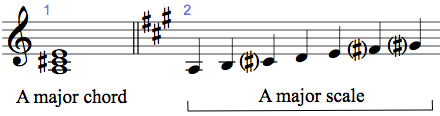
\includegraphics[scale=0.6]{chord-scale}
\caption{chord-scale duality.}
\end{figure*}


\subsection{The triad and harmonic analysis}

Each scale degree of a major or minor scale can support a triad constructed from the pitches of the scale. In Roman numeral analysis, each of these triads can be identified with a Roman numeral, and more complex chords can be analyzed based an underlying triad and figured bass to denote inversions \citep[pg.~68-9]{laitz2008}. For example, in the key of A major, the A major triad \{A, C$\sharp$, E\} is assigned \rom{1} and an E dominant 7th chord \{E, G$\sharp$, B, D\} is assigned \rom{5}$^7$ based on the E major triad, notated as \rom{5}. Roman numeral analysis is powerful because it focuses on the harmonic information stored in triads. Tonic and dominant triads alone can establish a key, as well as a sense of resolution as the harmony returns to the tonic \citep[pg.~103]{laitz2008}. From a theorist's standpoint, this means that chords must be analyzed within the context of the chords that come before and after. The tonic chord is the ultimate goal of any harmonic motion, and the relationship between the tonic and dominant chords generates the tension-resolution dynamic that propels music forward \citep[pg.~106]{laitz2008}. \textit{Cadences} often represent the most definitive harmonic indicators because they define points of resolution in music. By establishing future expectation The final chords leading to a resolution are known as a cadence. The authentic cadence \rom{4}-\rom{5}-\rom{1} is the strongest form of resolution in tonal harmony (\textbf{get a scholar to talk about cadences}). \\


\subsection{Bach's settings of the chorales}

A \textit{chorale} is a congregational hymn that first came into use during the early decades of the German Protestant Reformation, under Martin Luther. These hymns were composed as a melody with lyrical text, and typically the composer drew heavily (if not outright stole) from existing secular songs, medieval Gregorian chant, and other sacred works to create their own chorales. The Baroque composer J.S. Bach contributed a few original melodies to the chorale corpus. However, his most important contribution to the chorale remains his harmonizations of hundreds of chorales in larger vocal and instrumental compositions, which were inserted into many of his works, including the St. Matthew Passion and the cantatas \citep{leaverchorale}. In particular, his harmonization of four-voice chorales - of which 341 exist in the well-known Riemenschneider collection - are masterful studies in counterpoint and the task of re-harmonizing a melody, and they remain a guide for modern church musicians, jazz writers, arrangers and students alike. This is due to the conventions Bach established for four-part voice writing regarding voice leading, cadential movement, and intervallic relationships between voices. In this paper, I examine the task of harmonizing a chorale melody by training a neural network to learn the generative grammar that Bach pioneered through his own harmonizations. \\

The four-voice chorale is written for the four standardized voice ranges: soprano, alto, tenor, and bass. The original chorale melody is given to the soprano, while the lower voices collectively represent the \textit{harmonization} of the melody. The form of the work is simple, typically a single iteration of the melody that is segmented into shorter phrases by a series of \textit{fermatas} that indicate a pause and point of emphasis. \footnote{ Grab information from Music 51 } The chorale must be viewed in a variety of dimensions. In the vertical dimension, the notes of each voice at time $t$ can be heard simultaneously as a chord; and by consequence, a chorale represents a four-voice chord progression. That progression is primarily guided by the cadences that structure each phrase, and each cadence is defined by the relationship between the melody and the bass line. The inner voices play a largely supportive role by increasing the complexity of the chords. In the linear dimension, the chorale is a combination of four independent melodic lines, and the contour of each line is governed by the conventions of \textit{voice leading}. Voice leading embodies a broad set of characteristics, but they include rules about preferred and undesired intervals, parallel and contrary motion, and methods for rhythmically embellishing a chord progression (i.e. passing tones). \\

\begin{figure*}[h]
\caption{ The opening of the chorale \textit{Nun lob' mein' Seel', den Herren} }
\centerline{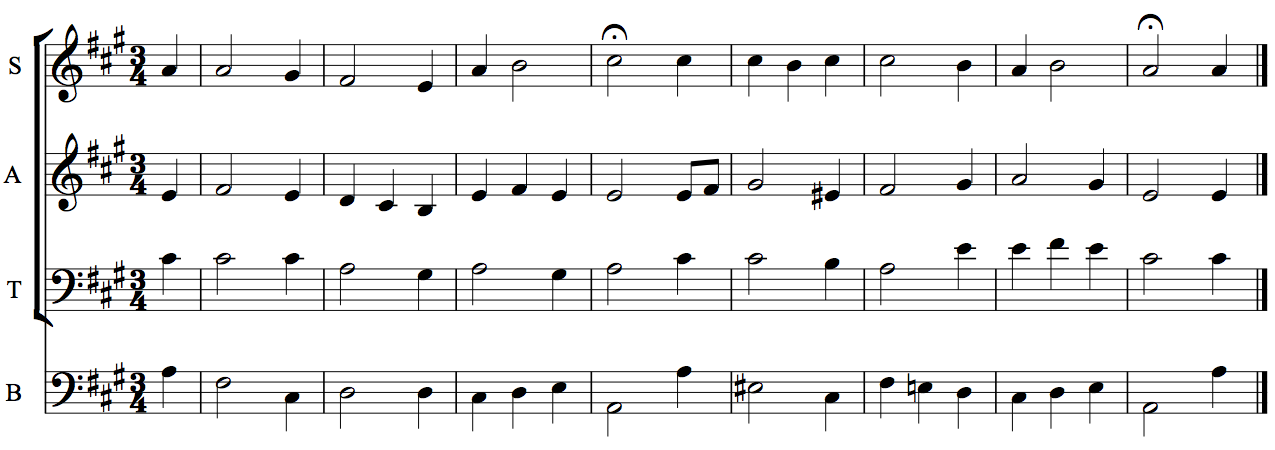
\includegraphics[scale=0.9]{chorale}}
\end{figure*}

The opening phrases of the chorale \textit{Nun lob' mein' Seel', den Herren} illustrate the importance of context in the task of harmonization. An important property of Bach's four-voice chorales is that the harmonic transitions occur very uniformly on each beat, so the task of harmonizing a chorale can be into divided into a time series of decisions for each beat of the melody. Bach's choice of harmonization for each beat is not a localized decision, but rather a decision that factors in information about the harmonic progression that preceded the current moment as well as the likely harmonies to occur next. For example, in measures 3-4 and measures 7-8, Bach constructs the cadence \lrom{2}$^6$ - \rom{5} - \rom{1}. Were we harmonizing the chorale ourselves in the same way and decided to harmonize the melody with a \lrom{2}$^6$ voicing on beat 2, this constrains the harmonies we could convincingly assign to beat 3. An additional constraint is placed by the fermata that occurs two beats later, which is almost certainly the resolution point of an authentic (\rom{1}) or half (\rom{5}) cadence. The harmonization of beat 3 must therefore bridge its surrounding harmonies to satisfy the expression \lrom{2}$^6$ - * - \{\rom{1}, \rom{5}\}. \\ 

Another important harmonic choice to examine is the C$\sharp^7$ harmony in measure 5, which is not diatonic to the chorale's key of A-major. In this case, C$\sharp^7$ functions as a secondary dominant, since the harmony resolves to $F\sharp$-minor in measure 6, and in f$\sharp$, C$\sharp^7$ is the dominant 7th chord. Secondary dominants are an effective tool for prolonging the resolution towards a certain harmony, and Bach uses them frequently to expand his harmonic pallette. The chorale \textit{Warum betr�bst du dich, mein Herz} illustrates the use of secondary dominants to facilitate a chromatically ascending bass line. \footnote{This is not my diagram, but will be replaced with my own (and my own Roman numeral analysis). Current image credited to \url{https://lukedahn.wordpress.com/2010/02/08/bachs-12-tone-chorale-phrases/}.} \\

\begin{figure*}[h]
\caption{ First phrase of \textit{Warum betr�bst du dich, mein Herz} }
\centerline{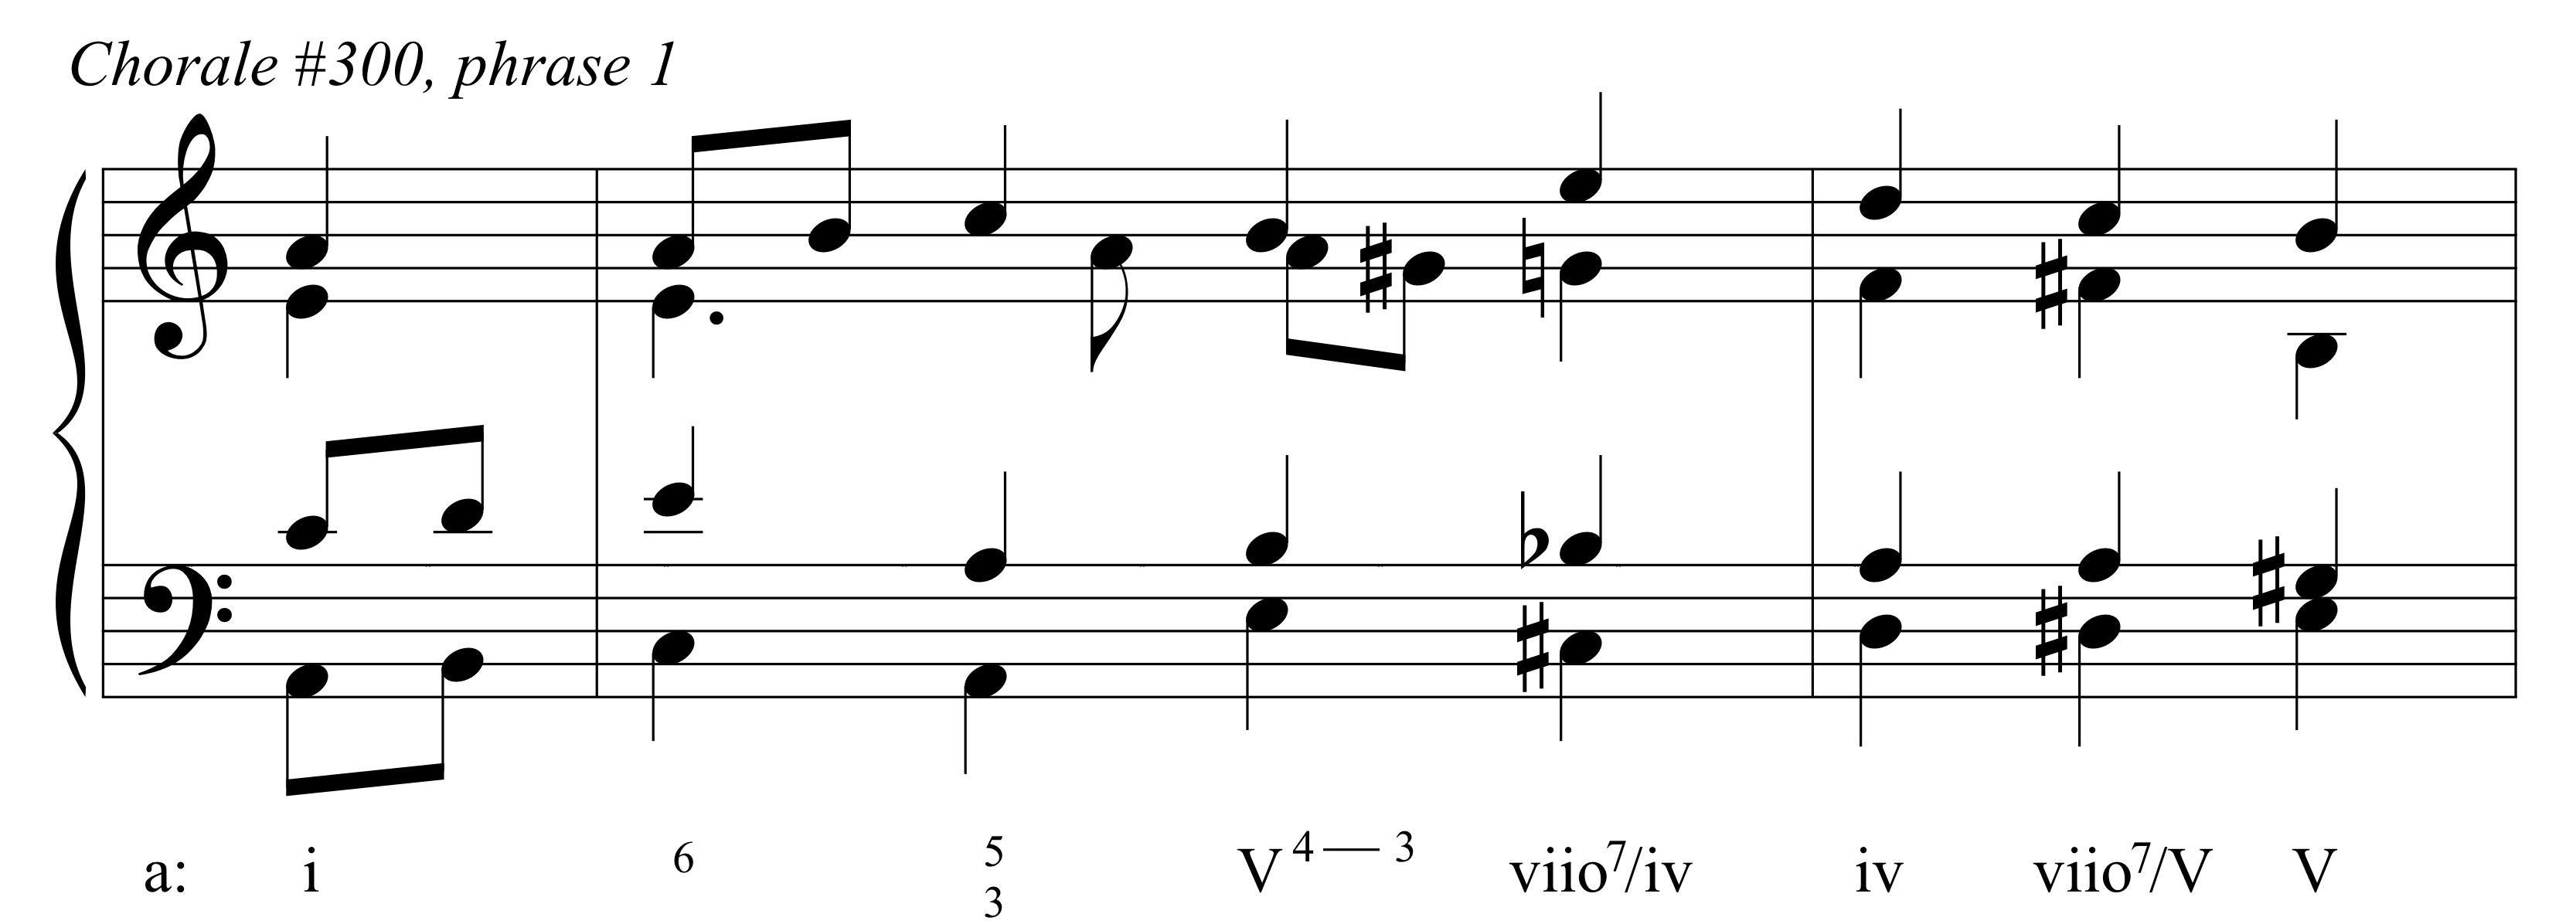
\includegraphics[scale=0.9]{chorale2}}
\end{figure*}

Therefore, a substantial model for chorale harmonization requires a variety of past, present, and future information in order to make accurate decisions. Characteristics of the melody note - such as pitch, beat strength, or the presence of a fermata - provide information about the stability of the harmony and whether or not a transitional harmony is more appropriate (such as a secondary dominant). The preceding harmonies indicate whether larger harmonic progressions are taking place, such as cadences and prolongations of a single harmony. And information about future events like fermatas or the final beat signal the endpoint of the current phrase, and so a convincing harmonic progression should lead towards the point of resolution.

\subsection{Exploratory Application: Bach Inventions}

The task of harmonization over a chorale is increasingly well-understood, particularly in the past few years with improved neural network architectures (\cite{greff2015lstm}; \cite{goel2014polyphonic}; \cite{liu2014Bach}). RNNs have also demonstrated their applicability to related musical tasks, such as the generation of a melody over a chord progression (\cite{franklin2006jazz}; \cite{eck2002blues}). Success in both of these areas suggests that this model is extensible to similar harmonization tasks, include those that require a higher degree of creativity than the strictly-rule based writing of four-voice counterpoint found in the chorales. Bach's 2-voice inventions, of which he composed 15, provide an excellent study of another harmonization task that applies similar rules of counterpoint between voices but introduces new complexities. The form on a invention, in particular, is more complicated than the chorale, the latter consisting of a short series of homophonic phrases. The piece can have one of a few loosely defined forms. Conventionally, the upper voice introduces the primary \textit{motive} - a melodic idea that establishes the primary melodic and rhythmic material for the work - while the left hand supports it in counterpoint and/or presents the motive in its own range. Each section of the work that introduces the motive is known as a \textit{presentation}. In between presentations, are \textit{episodes}, which are typically harmonically sequential material. A more free-form codetta often concludes the piece that provides the final harmonic closure.

The upper voice, is the leading voice of the work, both because it originally presents the motive and by nature of the conventional role of the right hand as the dominant hand. As a result, the lower voice can be viewed as a supporting character, echoing the melodic material of its counterpart and providing harmonic support elsewhere. The lower voice is a function of the upper voice, and therefore the new task is defined as follows: given the upper voice of the invention, compose the lower voice.   

\begin{figure*}[h]
\caption{ The opening measures of Invention $\sharp$1 in C-Major. }
\centerline{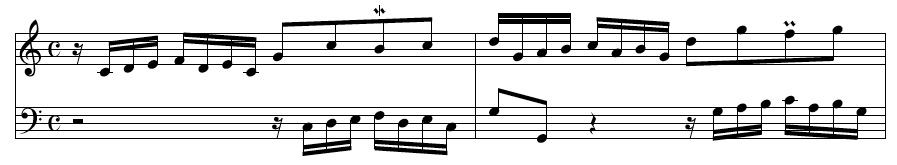
\includegraphics[scale=0.5]{invention1}}
\end{figure*}

Figure 8 illustrates the presentation of the motive in the upper voice, followed by an echo of the motive shortly after in the left hand. In this invention and many others, the motive is presented without much ornamentation in the opening measures so that in later presentations, the motive can be transformed and altered in interesting ways while still preserving its original character. This means that from a computational point of view, we want to learn to focus on the opening measures of the upper voice since the original and un-ornamented presentation of the motive is the most important piece of information to understanding how the invention will develop. And using LSTM networks, the strong correlations between presentations can be learned despite their temporal distance. An important measure of success will be the model's ability to determine the important aspects of the form, which determine whether the lower voice should echo the upper voice melody or support in counterpoint.

Another form of additional complexity not found in the chorales is a diversity of rhythmic ideas. The works can no longer be divided into a time series of beats, but \textit{harmonies} tend to persist a minimum of a beat and typically two or more. Therefore, a potential preprocessing step would be to generate a harmonic skeleton for the work. The density of the upper voice in inventions actually provides significantly more harmonic information than the 3 or 4 notes per measure found in the soprano voice of the chorale. Another potential preprocessing step would be to search the upper voice for moments of repeated melodic content. By identifying these moments as presentations, the form of the work can be constructed around those moments.

\newpage

\printbibliography









\end{document}